%----------------------------------------------------------------------------------------
%	PACKETS AND CONFIGURATION
%----------------------------------------------------------------------------------------

\documentclass[11pt]{beamer}
\setbeamercovered{transparent}

\usepackage{title}  		% Title settings for the presentation
\usepackage{parskip}    	% Paragraph indent & skip
\usepackage{xcolor}     	% More colors
\usepackage{enumitem}		% Better lists
\usepackage{graphicx}  		% 'graphics' package interface
\usepackage{listings}   	% Code sections formatting}
%\usepackage{pdftexcmds}
%\usepackage{minted}
%\usepackage[utf8]{inputenc}
%\usepackage[T1]{fontenc}
%\usepackage{pythontex}
\usepackage{verbatim}

% Custom colors
\definecolor{AnnotationGreen}{RGB}{34, 128, 45}
\definecolor{CommentGreen}{RGB}{29, 204, 49}

% Python code formatting
% Use it by creating an environment like \begin{lstlisting}[style=Python] ... \end{lstlisting}
% Since annotations aren't tagged as keywords I have inserted a manual delimiter for them,
% it works as follows: \@@AnnotationText@@/
\lstdefinestyle{Python}{
    language = Python,
    basicstyle = \footnotesize\ttfamily,
    commentstyle = \textcolor{CommentGreen},
    stringstyle = \textcolor{orange},
    showstringspaces = false,
    keywordstyle = \textcolor{blue},
    moredelim = [is][\textcolor{AnnotationGreen}]{\\@}{@@\/},   % Annotations
    numberstyle = \scriptsize\ttfamily\textcolor{gray},
    numbers = left,
    frame = single,
    frameround = tttt,
    framexleftmargin = 10pt,
    framexrightmargin = 0pt
}

% HELPER PACKAGES (TODO: REMOVE IN FINAL) %
\usepackage{todonotes}
\presetkeys{todonotes}{inline}{}
\usepackage{blindtext}
% HELPER PACKAGES (TODO: REMOVE IN FINAL) %

\usetheme{Antibes} % THEME

%----------------------------------------------------------------------------------------
%	DOCUMENT
%----------------------------------------------------------------------------------------

\begin{document}

% TITLE
\frame{\titlepage}

% Table of Contents
\begin{frame}{Presentation Outline}
\begin{tiny}
    \tableofcontents[hideallsubsections]
\end{tiny}
\end{frame}

% Environment and Simulation ------------------------------------------------------------

\AtBeginSection[]
{
\begin{frame}{}
    \tableofcontents[sections={\thesection}]
\end{frame}
}

% ----------------------------------------

\section{Introduction}

%-----------------------------------------

\begin{frame}

\frametitle{Project Scope}
\framesubtitle{Assignment}

The focus of this project is to optimize the budget allocated for the \textbf{advertisement campaigns} of 5 different items in order to maximize the profit of an \textit{e-commerce website} that sells products to the public.

Each page has a \textbf{primary product} and some \textbf{secondary products}, each user that lands on a page has a possibility to buy the primary prodcut and/or proceed to one of the secondaries with a given probability, the process repeats.

\end{frame}


%-----------------------------------------

\begin{frame}

\frametitle{Project Scope}
\framesubtitle{Techniques}

The optimization has to be perfomed on different scenarios and using different algorithms.

We had to direct our focus on bandit algorithms combining Gaussian Processes with Upper Confidence Bound and Thompson Sampling algorithms.

For each different scenario the performance of the learners based on these algorithm is evaluated against the Clayrvoiant and the Stupid Learner.

\end{frame}

%-----------------------------------------

\begin{frame}

\frametitle{General hypoteses}

The main general hypoteses that were given to us are:
\begin{itemize}[label={-}]
    \item For every \textit{primary product}, the \textit{secondary products} to display and their order is fixed.
    \item The price of every product is fixed and it is equal to the margin.
    \item By clicking on a specific ad, the user lands on the corresponding \textit{primary product}.
\end{itemize}

\end{frame}

% ----------------------------------------

\section{Environment and Simulation}

%-----------------------------------------

\subsection{Overview}

%-----------------------------------------

\begin{frame}

\frametitle{Assumptions}
\framesubtitle{E-commerce website}

For this project, we are required to design an \textbf{Environment} that satisfies various constraints both on the e-commerce site's properties and on the users' behavior; in addition, since most of the tasks were generic, we had to come up with some of our own assumptions.

In particular we want to underline the following assumptions for the e-commerce website:
\begin{itemize}[label={-}]
    \item The website has unlimited stock for the 5 different items.
    \item Actions on the various webpages are \textbf{perfectly observable} by the e-commerce website.
\end{itemize}

\end{frame}

% ----------------------------------------

\begin{frame}

\frametitle{Assumptions}
\framesubtitle{Users}

...and we assume that the users present the following behaviors:
\begin{itemize}[label={-}]
    \item Every day, there is a random number (subject to noise) of potential new users.
    \item The \textit{reservation price} for each user is always over the single unit. \todo{?}
    \item The users can activate parallel paths while on the website.
    \item The number of items that a user will buy is a random variable, independent from any other variable.
\end{itemize}

\todo{insert text somewhere}
%The behavior of a user is modelled as a graph where nodes represent product pages and weights represent the probabilities for the user to click from the primary item of the page to one of the secondaries.

\end{frame}

%-----------------------------------------

\subsection{Environment structure}

%-----------------------------------------

\begin{frame}[fragile]

\frametitle{Environment}
\framesubtitle{Structure}

The environment is modelled as a python dataclass containing the following attributes:

\begin{lstlisting}[style=Python, basicstyle=\tiny, numbers=none, framexrightmargin=-20pt]
    # The total budget to subdivide
    total_budget: int

    # Probability of every class to show up. They must add up to 1
    class_ratios: List[float]

    # Features associated to every class
    class_features: List[List]

    # Price of the 5 products
    product_prices: List[float]

    # List of class parameters for each class and product,
    # implemented as list of lists of UserClassParameters.
    # Each class has distinct parameters for every product
    classes_parameters: List[List[UserClassParameters]]
\end{lstlisting}

\end{frame}

% ----------------------------------------

\begin{frame}[fragile]

\frametitle{Environment}
\framesubtitle{Structure}

\begin{lstlisting}[style=Python, basicstyle=\tiny, numbers=none, framexrightmargin=-20pt]
    # Lambda parameter, which is the probability of osserving the
    # next secondary product according to the project's assignment
    lam: float

    # Max number of items a customer can buy of a certain product.
    # The number of bought items is determined randomly with
    # max_items as upper bound
    max_items: int

    # Products graph's matrix. It's a empty matrix, should be
    # initialized with populate_graphs
    graph: np.ndarray

    # List that constains for every i+1 product the secondary i+1
    # products that will be shown in the first and second slot
    next_products: List[Tuple[int, int]]

    # Controls randomness of the environment
    random_noise: float
\end{lstlisting}

\end{frame}

% ----------------------------------------

\begin{frame}

\frametitle{Environment}
\framesubtitle{Masked Environment}

Alongside the \textbf{Environment} we define a \textbf{Masked Environment} with the purpose of \textit{hiding crucial information} to the learners since each type of learner should only have access to a subset of all the information available in the environment dictated by the type of learner.

The masked environment isn't strictly needed in the project since the learners could easily ignore the extra information, however, we wanted to face the problem with an approach aimed towards reusability and extendability and in this case (as in many others down the line) we opted for a more \textbf{generalizable} solution.

\todo{we talk about learners without metioning them before, we need to introduce them in the introductory section}

\end{frame}

% ----------------------------------------

\begin{frame}

\frametitle{Users}
\framesubtitle{User parameters}

We modelled the $\alpha$-functions, which compute the expected value of interactions on a product given a fixed budget, as \textbf{exponential functions}.

In particular their \textit{upper bound} represents the maximum expected number of interactions possible while the \textit{maximum useful budget} is the amount of budget after which any budget increase would not lead to a ratio increase.

\end{frame}

% ----------------------------------------

\begin{frame}

\frametitle{Users}
\framesubtitle{User classes}

\begin{itemize}[leftmargin=*, label={$\circ$}]
    \item Users are subdivided in classes based on their \textit{2 binary features} for a total of \textit{3 different classes}.
    \item In particular, each user class is defined by its $\alpha$-functions (one for each product plus the one for the non-strategic competitor) which define the probability of landing on a given product page.
    \item Each $\alpha$-function is defined by the values: \textbf{reservation price}, \textbf{upper bound} and \textbf{maximum useful budget}
\end{itemize}

\end{frame}

% ----------------------------------------

\subsection{Randomness in the Environment}

% ----------------------------------------

\begin{frame}

\frametitle{Randomness in the Environment}
\framesubtitle{Non determinism}

\begin{itemize}[leftmargin=*, label={$\circ$}]
    \item For the sake of representing a real scenario, most of the values that are not known a priori are \textit{randomly generated} and every variable that evolves through time without our direct control has elements of randomness to it (for instance, each day we randomly get the number of active total users in our scenario by using a gaussian distribution with tunable mean and standard deviation).
    \item Even though most of the randomness is tunable and controlled through seeded generators, there are still \textbf{impactful elements of non determinism} (i.e. the Dirichlet distribution) that are not possible to control in any way.
\end{itemize}

\end{frame}

% ----------------------------------------

\begin{frame}

\frametitle{Randomness in the Environment}
\framesubtitle{Consequences}

\todo{how does non determinism affect clairvoyant results?}

\end{frame}

% ----------------------------------------

\subsection{Simulation}

% ----------------------------------------

\begin{frame}

\frametitle{Daily Simulation}
\framesubtitle{Purpose}

\begin{itemize}[leftmargin=*, label={$\circ$}]
    \item The \textbf{Simulation} class is the main engine that brings together \textit{learners} and \textit{environment} by making them interact with each other while offering an interface to customize the execution.
    \item The basic idea of the simulation is to simulate a real scenario day by day using the environment to generate interactions with the website according to the budgets that the current learner proposed and then, feed the results back to the learner to make it actually learn.
    \item Repeating the simulation execution step for each day until an arbitrary \textbf{time horizon} is reached grants us all the data needed to evaluate the performance of our learner.
\end{itemize}

\end{frame}

% ----------------------------------------

\begin{frame}

\frametitle{Daily Simulation}
\framesubtitle{Example}

\todo{insert generic learner execution plot over n days}

\end{frame}

% Optimization Algorithm ----------------------------------------------------------------

\AtBeginSection[]
{
\begin{frame}{}
    \tableofcontents[sections={\thesection}]
\end{frame}
}

% ----------------------------------------

\section{Optimization Algorithm}

% ----------------------------------------

\subsection{General Problem}

% ----------------------------------------

\begin{frame}

\frametitle{Problem formulation}

The purpose of the \textbf{optimization algorithm} is to find the \textit{optimal budget} for each campaign in order to maximize the \textit{profit}, which is defined as the difference between the profits gained from selling products and the advertisement expenses.
Basically, it is a maximization problem subject to an obvious constraint: the sum of the daily budget can't be greater then the overall budget.

The optimization problem can be expressed as follows:
\begin{displaymath}
F=\max_{\substack{x_i\in B}} \sum_{i=0}^n \alpha_i(x_i)p_i-x_i \ s.t. \sum_{i=0}^n x_i\leq B
\end{displaymath}

\end{frame}

% ----------------------------------------

\subsection{Algorithm}

% ----------------------------------------

\begin{frame}

\frametitle{Code}
\framesubtitle{Functioning}

\todo{talking about the code in words}

\end{frame}

% ----------------------------------------

\begin{frame}

\frametitle{Code}
\framesubtitle{Example}

\todo{snippets of code}

\end{frame}

% Uncertain alpha functions -------------------------------------------------------------

\AtBeginSection[]
{
\begin{frame}{}
    \tableofcontents[sections={\thesection}]
\end{frame}
}

% ----------------------------------------

\section{Uncertain $\alpha$-functions}

% ----------------------------------------

\subsection{Contextual hypotesis}

% ----------------------------------------

\begin{frame}

\frametitle{Uncertain $\alpha$-functions}
\framesubtitle{Scenario}

We assume now that the binary features of the users cannot be observed and therefore data are aggregated.

\end{frame}

% ----------------------------------------

\subsection{Algorithm}

% ----------------------------------------

\begin{frame}
\frametitle{Uncertain $\alpha$-functions}
\framesubtitle{Algorithm}

Since the feature of the users are \textbf{not observable}, the algorithm receives all the interactions minus the class data.
It tries to estimate the reward given by each single product.

\end{frame}

% ----------------------------------------

\begin{frame}

\frametitle{Uncertain $\alpha$-functions}
\framesubtitle{Result}
\todo{: going to insert some graph of clayrvoiantv stupid}

\end{frame}

% Uncertain alpha functions and number of items sold ------------------------------------

%\section{Uncertain $\alpha$-functions and number of items sold}

% Uncertain graph weights ---------------------------------------------------------------

%\section{Uncertain Graph Weights}

% Non-stationary demand curve -----------------------------------------------------------

\AtBeginSection[]
{
\begin{frame}{}
    \tableofcontents[sections={\thesection}]
\end{frame}
}

% ----------------------------------------

\section{Non-stationary demand curve}

% ----------------------------------------

\subsection{Environment behavior}

% ----------------------------------------

\begin{frame}
\frametitle{Non-stationary behavior}
\framesubtitle{Overview}

By using the \textbf{non-stationarity} assumption we are taking into consideration that the demand curve could be subject to changes over time and isn't necessarily fixed as we have seen in other steps.

There are 2 main types of \textit{non-stationary behaviors}:
\begin{itemize}[label={$\circ$}]
    \item \textbf{Abrupt changes}: where it's possible to identify different phases with different phase-wise stationary demand curves.
    \item \textbf{Smooth changes}: where the demand curve changes over time in a continuous manner.
\end{itemize}

As per specifications, we will only consider \textbf{abrupt changes} in the scope of our project.

\end{frame}

% ----------------------------------------

\begin{frame}
\frametitle{Non-stationary behavior}
\framesubtitle{Abrupt changes}

\textbf{Abrupt changes} are usually experienced when an important event strikes the market \textit{(e.g. a new product that shifts the interests of the users is released or an historical event shapes the opionion of people)}; change isn't necessarily bad, however, it may impact negatively the prediction of learners that were created with a static environment in mind.

Neither \textbf{UCB1} nor \textbf{TS} account for abrupt changes since it's almost impossible for them to try a superarm that was deemed as \textit{unoptimal} over the past iterations (while it might have become optimal after an \textit{abrupt change}), therefore we expect to see a significant \textbf{reward drop} from them after an \textit{abrupt change}.

\end{frame}

% ----------------------------------------

\begin{frame}
\frametitle{Simulating abrupt changes}

In the early stages of the project we noticed that the \textbf{Simulation} that we created wasn't really fit to dinamically include abrupt changes in the environment, therefore great effort was spent in completely reworking the interface for the \textbf{Simulation} from the ground-up.

Besides collateral improvements in reproducibility, results collection and user-friendliness, the new \textbf{Simulation} allowed for an \textit{incremental simulation unfolding}, this meant that we were now able to simulate \textit{n} days, change the environment and simulate another \textit{n} days.

This particular feature revealed itself as fundamental for the upcoming challenges.

\end{frame}

% ----------------------------------------

\subsection{Algorithms}

% ----------------------------------------

\begin{frame}
\frametitle{Approaches}
\framesubtitle{Sliding window and Change detection}

There are 2 main approaches to deal with a \textbf{non-stationary environment}
\begin{itemize}[label={$\circ$}]
    \item \textbf{Sliding window}: only consider the last $\tau$ samples for predictions.
    \item \textbf{Change detection}: detect when a change has happened and adapt accordingly.
\end{itemize}

It's clear that \textbf{Sliding window} approaches are more fit for \textbf{smooth changes} while \textbf{Change detection} approaches work better with \textbf{abrupt changes}, however it's important to note that both approaches can be utilized to deal with any \textit{non-stationary} scenario.

\end{frame}

% ----------------------------------------

\begin{frame}
\frametitle{Sliding window}
\framesubtitle{Sliding window for TS and UCB1}

\begin{itemize}[leftmargin=*, label={$\circ$}]
    \item \textbf{SW-UCB1} differs in the confidence bound formulation and the new arm choice:
        \begin{displaymath}
            a_t =
            \begin{cases}
                a_{\overline{t}} & \text{if} ~ \exists \overline{t} \vert n_{a_{\overline{t}}}(t-1, \tau) = 0 \\
                arg\max\limits_{a \in A} \left\{ \overline{x}_{a, t, \tau} + \sqrt{\frac{2log(t)}{n_a(t-1, \tau)}} \right\} & \text{otherwise}
            \end{cases}
        \end{displaymath}
    \item \textbf{SW-TS} differs in the $\beta$ distribution update:
        \begin{displaymath}
            \displayindent0pt \displaywidth\textwidth
            (\alpha_{a_t}, \beta_{a_t}) =
            \begin{cases}
                (\alpha_{a_t}, \beta_{a_t}) + (x_{a_t, t}, 1-x_{a_t, t}) & \text{if} ~ t \leq \tau \\[1ex]
                \!\begin{aligned}
                    & \max \{ (1, 1)\!\begin{aligned}[t]
                        & , (\alpha_{a_t}, \beta_{a_t}) + (x_{a_t, t}, 1-x_{a_t, t}) \\
                        & - (x_{a_{t-\tau}, t-\tau}, 1-x_{a_{t-\tau}, t-\tau}) \}
                    \!\end{aligned}
                \end{aligned} & \text{if} ~ t > \tau
            \end{cases}
        \end{displaymath}
\end{itemize}

\end{frame}

% ----------------------------------------

\begin{frame}
\frametitle{Change detection}

We used a \textbf{reward-based algorithm} as a \textit{change detection algorithm}, it works by comparing the last $k$ rewards with the newest $k$ rewards ($k=4$ by default) and if the difference between their means exceedes a certain threshold $\omega$ ($\omega=400$ by default) the learner is \textbf{reset} and is therefore able to learn a new optimal superarm from scratch.

Formally:
\begin{displaymath}
    \text{RESET learner if} ~ t \geq 2k ~ \land \sum_{i=t-2k}^{t-k} r_i -\sum_{i=t-k+1}^t r_i > \omega
\end{displaymath}

\scriptsize N.B. there is an offset of 1 in the representation of t between theory and code

\end{frame}

% ----------------------------------------

\subsection{Results}

% ----------------------------------------

\begin{frame}
\frametitle{}
\framesubtitle{}

\todo{insert correct image}
%\makebox[\textwidth]{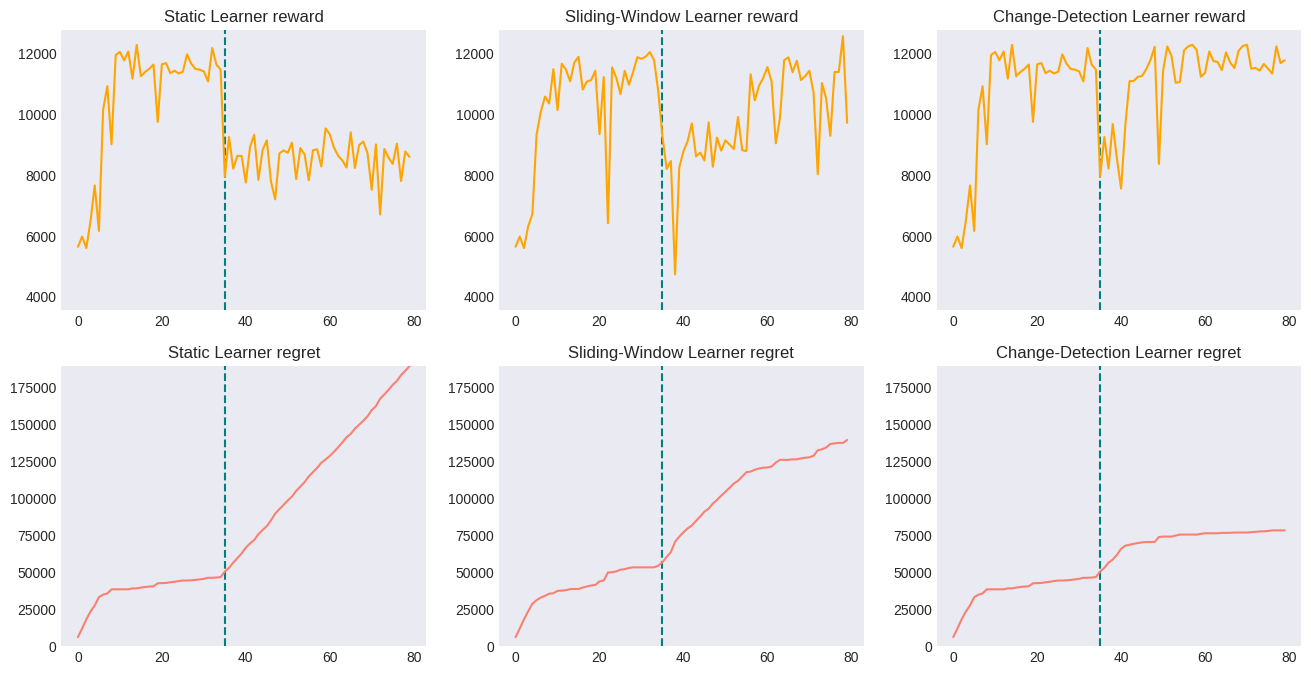
\includegraphics[width=\paperwidth]{img/step6/image1.png}}

\scriptsize Graphs representing reward and regret in the non-stationary environment with different approaches. (Only \textbf{UCB1} algorithms were evaluated)

\end{frame}

% ----------------------------------------

\begin{frame}
\frametitle{Reward and regret}

We calculated the mean \textbf{reward} and \textbf{regret} considering their variance over multiple runs.

\todo{insert image}
%\makebox[\textwidth]{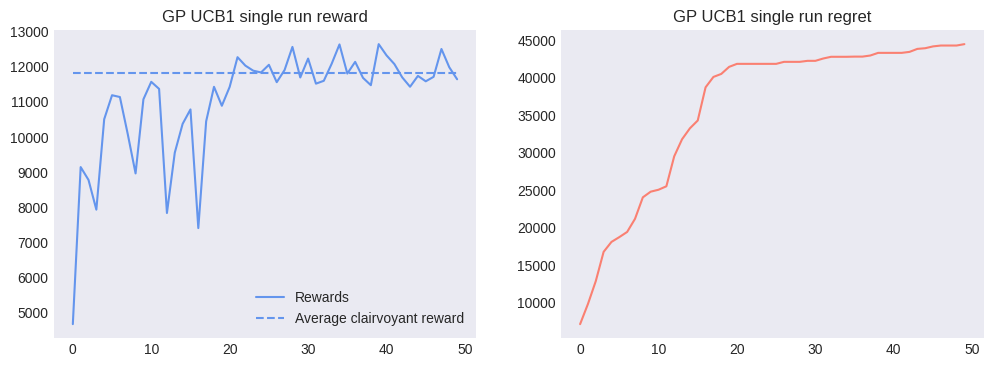
\includegraphics[width=\paperwidth]{img/step6/image2.png}}

\end{frame}

% ----------------------------------------

\begin{frame}
\frametitle{Theoretical guarantees}

In addition, if the \textbf{number of breakpoints} $m$ is small enough with respect to the \textbf{time horizon} $T$ to the power of $\alpha$ we have that the \textbf{regret} is of the order $O\left( \vert A \vert T^{\frac{1+\alpha}{2}} \right)$

\end{frame}

% Context generation --------------------------------------------------------------------

%\section{Context generation}

\end{document}


%NOTE TO US:
%%\centering if we want the presentation to be power-point style
